\section{MJD Waveform Evidence for Energy-Aware Evaluation}
\label{app:mjd-motivation}

\paragraph{Task, population, and selection.}
The local MJD release contains six test shards with 390,000 events,
including 148,251 clean events. Clean means that all four reference PSD
labels---low AvsE, high AvsE, DCR, and LQ---equal one; the formal task is
clean versus non-clean, not low versus high energy. Calibrated energy is
provided by \texttt{energy\_label} in keV, and raw waveforms contain 3800
ADC samples \citep{arnquist2023mjdrelease}. We choose the detector/run pair
with the most clean test events, breaking count ties by detector and run
identifier. This gives detector 133, run 50928, with 410 events. Selection
uses metadata and labels, before waveform inspection.

The lower and upper energy quartile boundaries are 226.871 and
471.248\,keV. The corresponding cohorts contain 103 events each,
covering 5.7--226.9 and 471.2--2616.4\,keV; the middle group contains 204.
For the event displays, we choose the event nearest each cohort's median
energy, with event identifier and row index breaking ties. The selected
events have energies 157.975 and 1131.515\,keV and identifiers 2407207
and 2585508. This rule does not inspect pulse shape or noise.

\paragraph{Actual waveform preprocessing.}
For raw waveform samples $v_{it}$, with $t=0,\ldots,3799$, define
\begin{equation}
 b_i=\frac{1}{200}\sum_{t=0}^{199}v_{it},\qquad
 \alpha_i=\max_t|v_{it}-b_i|,\qquad
 u_{it}=\frac{v_{it}-b_i}{\alpha_i}.
\end{equation}
The implementation reads float32 samples, computes the baseline mean in
float64 and casts it to float32, then subtracts and normalizes in float32.
Division is skipped when $\alpha_i=0$; no selected event has zero amplitude.
This is the common waveform preparation before the STFT or point
representation, not an assertion that every classifier directly receives
the plotted one-dimensional array. The time axis is sample index; no
sampling interval is assumed.

We summarize residual baseline fluctuations by
\begin{equation}
 r_i=\left(\frac{1}{200}\sum_{t=0}^{199}u_{it}^2\right)^{1/2}.
\end{equation}
Up to float32 rounding, $r_i$ is baseline RMS in ADC counts divided by
$\alpha_i$. It is a descriptive input statistic, distinct from the benchmark's
energy independence score. The lowest/highest energy cohorts have median
$r_i$ values 0.006720 and 0.000889, a ratio of 7.56. Their absolute baseline
RMS medians are much closer, 2.233 and 2.166 ADC counts. Across the 410
events, energy has Spearman correlation 0.993 with $\alpha_i$, $-0.012$ with
absolute baseline RMS, and $-0.826$ with $r_i$. These are single-cohort
descriptive statistics, without uncertainty intervals or a claim that
they hold for every detector/run. Neither correlation nor these event
displays determines the strategy of a trained classifier.

\begin{figure}[!htb]
\centering
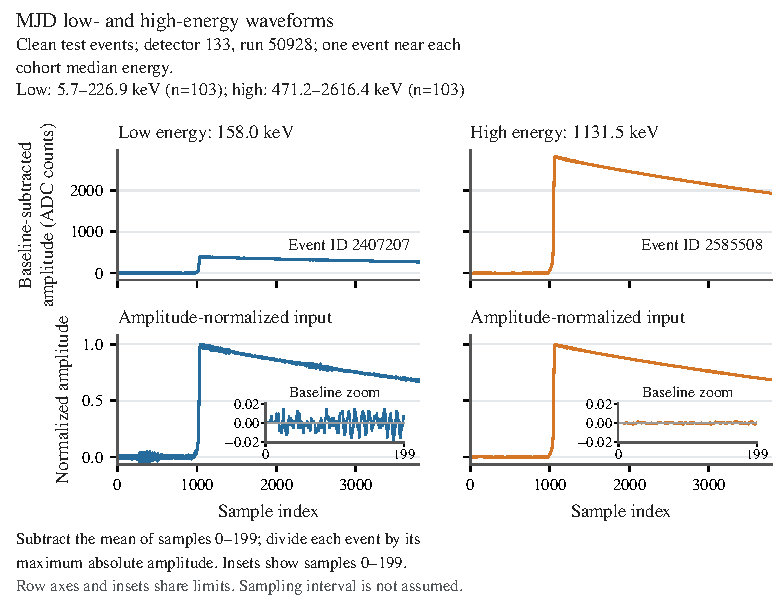
\includegraphics[width=.95\linewidth]{wing_contribution/figures/mjd_low_high_waveforms.pdf}
\caption{Detailed MJD event displays from the fixed detector/run cohort.
Top: baseline-subtracted ADC amplitudes. Bottom: normalized waveforms
before model-specific representation, with enlarged first-200-sample
baselines. The two columns share vertical limits within each row, and
both baseline insets use the same scale. Events were selected by energy
alone using the stated median rule.}
\label{fig:mjd-waveform-details}
\end{figure}

\paragraph{Connection to the saved benchmark.}
Raw test labels and event IDs match the saved CNN evaluation population.
Calibrated energies are recovered in float64 from the original test shards;
the old adapter's float32 conversion and clipping are not used. The 67 events
above 3000 keV (66 non-clean and one clean) are excluded from energy evaluation
before support estimation; they remain in the original coverage denominator.
The common support is $[18.151,2613.790]$ keV with 493 valid 5 keV bins,
retaining 146,383 clean and 232,824 non-clean events.
The CNN's inclusive and matched AUCs are 0.971283 and 0.969851, respectively,
while $I=0.759637$. The small AUC difference does not establish
energy-dominated classification. Matching controls the class energy
mixture; the independence score asks a separate question about the
predictions within each class.
